En el presente documento se explicará cómo hacer uso de las diferentes herramientas que se han utilizado a lo largo del desarrollo del sistema inteligente de detección de señales. Destacar que el desarrollo ha sido llevado a cabo en un ordenador con sistema operativo \textit{MAC OS/Linux}, es decir, en caso de trabajar con un ordenador \textit{Windows} habrá que prestar especial al código. Tendrás que modificar las líneas en las que se hace referencia a directorios o ficheros, ya que se hace de forma diferente en dichos sistemas operativos, en \textit{MAC OS/Linux} se hace con \textbf{‘/’} y en \textit{Windows} con \textbf{‘\textbackslash ’}. Asimismo, los directorios están referenciados respecto a nuestro ordenador personal, por lo que habrá que adecuarlos al tuyo propio.\\

Para hacer uso del sistema, debemos descargarnos el proyecto de nuestro repositorio de \textit{GitHub}, suponiendo que tenemos la herramienta de línea de comandos de \textit{git} instalada, podemos hacer:\\

\begin{lstlisting}
git clone https://github.com/OscarMartinn/TallerDeProyectos2.git
\end{lstlisting}

En primer lugar, para poder trabajar con todo proyecto debemos crear nuestro propio entorno virtual en el cual instalaremos todas las librerías necesarias para ejecutar el código. 

\begin{lstlisting}
python3 -m venv 'nombre_entorno'
\end{lstlisting}

Una vez creado el entorno debemos activarlo, por ejemplo, en un ordenador \textbf{MAC}:

\begin{lstlisting}
source nombre_entorno/bin/activate
\end{lstlisting}

Todas las librerías necesarias junto con sus versiones concretas se han guardado en el fichero \textit{requirements.txt}, por ello instalaremos automáticamente cada una de ellas:

\begin{lstlisting}
pip install -r requirements.txt
\end{lstlisting}

Tras realizar todos los pasos anteriores ya nos encontramos en disposición de ejecutar todos los algoritmos.\\
Desglosaremos el proyecto en tres partes distintas:
\begin{enumerate}
\item Detección y seguimiento de señales
\item Herramienta de etiquetado
\item Medición del rendimiento
\item Creación automática de datasets.
\end{enumerate}

\subsection{Detección y seguimiento de señales}	
	Accediendo a la primera carpeta \textbf{1_YOLOV3} nos encontraremos con todos los scripts encargados de ejecutar el algoritmo. Tenemos cinco ficheros \textbf{Python}:

\begin{enumerate}
\item \textbf{imagen_yolov3.py}: script encargado de detección de señales en una imagen individual.
\item \textbf{video_yolov3.py}: script encargado de detección de señales en un video.
\item \textbf{camara_yolov3.py}: script encargado de detección de señales a través de la cámara frontal o webcam del ordenador.
\item \textbf{automatic_imagen_yolov3.py}: script encargado de detección de señales en una imagen individual, pero el nombre de la imagen a procesar se introducirá mediante línea de comandos y no dentro del fichero.
\item \textbf{automatizacion_imagenes.py}: script encargado de leer todas las imágenes de un directorio y mandárselas a través de línea de comandos al fichero \textit{automatic_imagen_yolov3.py} para poder procesar varias imágenes ininterrumpidamente.
\end{enumerate}

Por la propia estructura de \textbf{YOLOV3}, todos los scripts encargados de la detección de señales se nutren de tres ficheros básicos, los que se encuentran dentro de la carpeta \textbf{yolo_data}:
\begin{itemize}
\item \textbf{classes.names}: fichero que contiene todas las clases de señales con las que ha sido entrenado el modelo y que va a ser capaz de detectar.
\item \textbf{yolov3_ts_test.cfg}: fichero que contiene la configuración de \textbf{YOLO}.
\item \textbf{yolov3_ts.weights}: fichero que contiene los pesos obtenidos como resultado del entrenamiento del modelo.
\end{itemize}

En el script \textbf{imagen_yolov3.py} deberemos modificar la variable \textit{imageName} con el nombre de la imagen en formato JPG, que ha de encontrarse dentro del directorio destinado a las imágenes \textit{images}. Con el siguiente comando podemos visualizar un ejemplo, figura \ref{detecc1} 

\begin{lstlisting}
python3 imagen_yolov3.py
\end{lstlisting}

\begin{figure}[H]
	\centering
	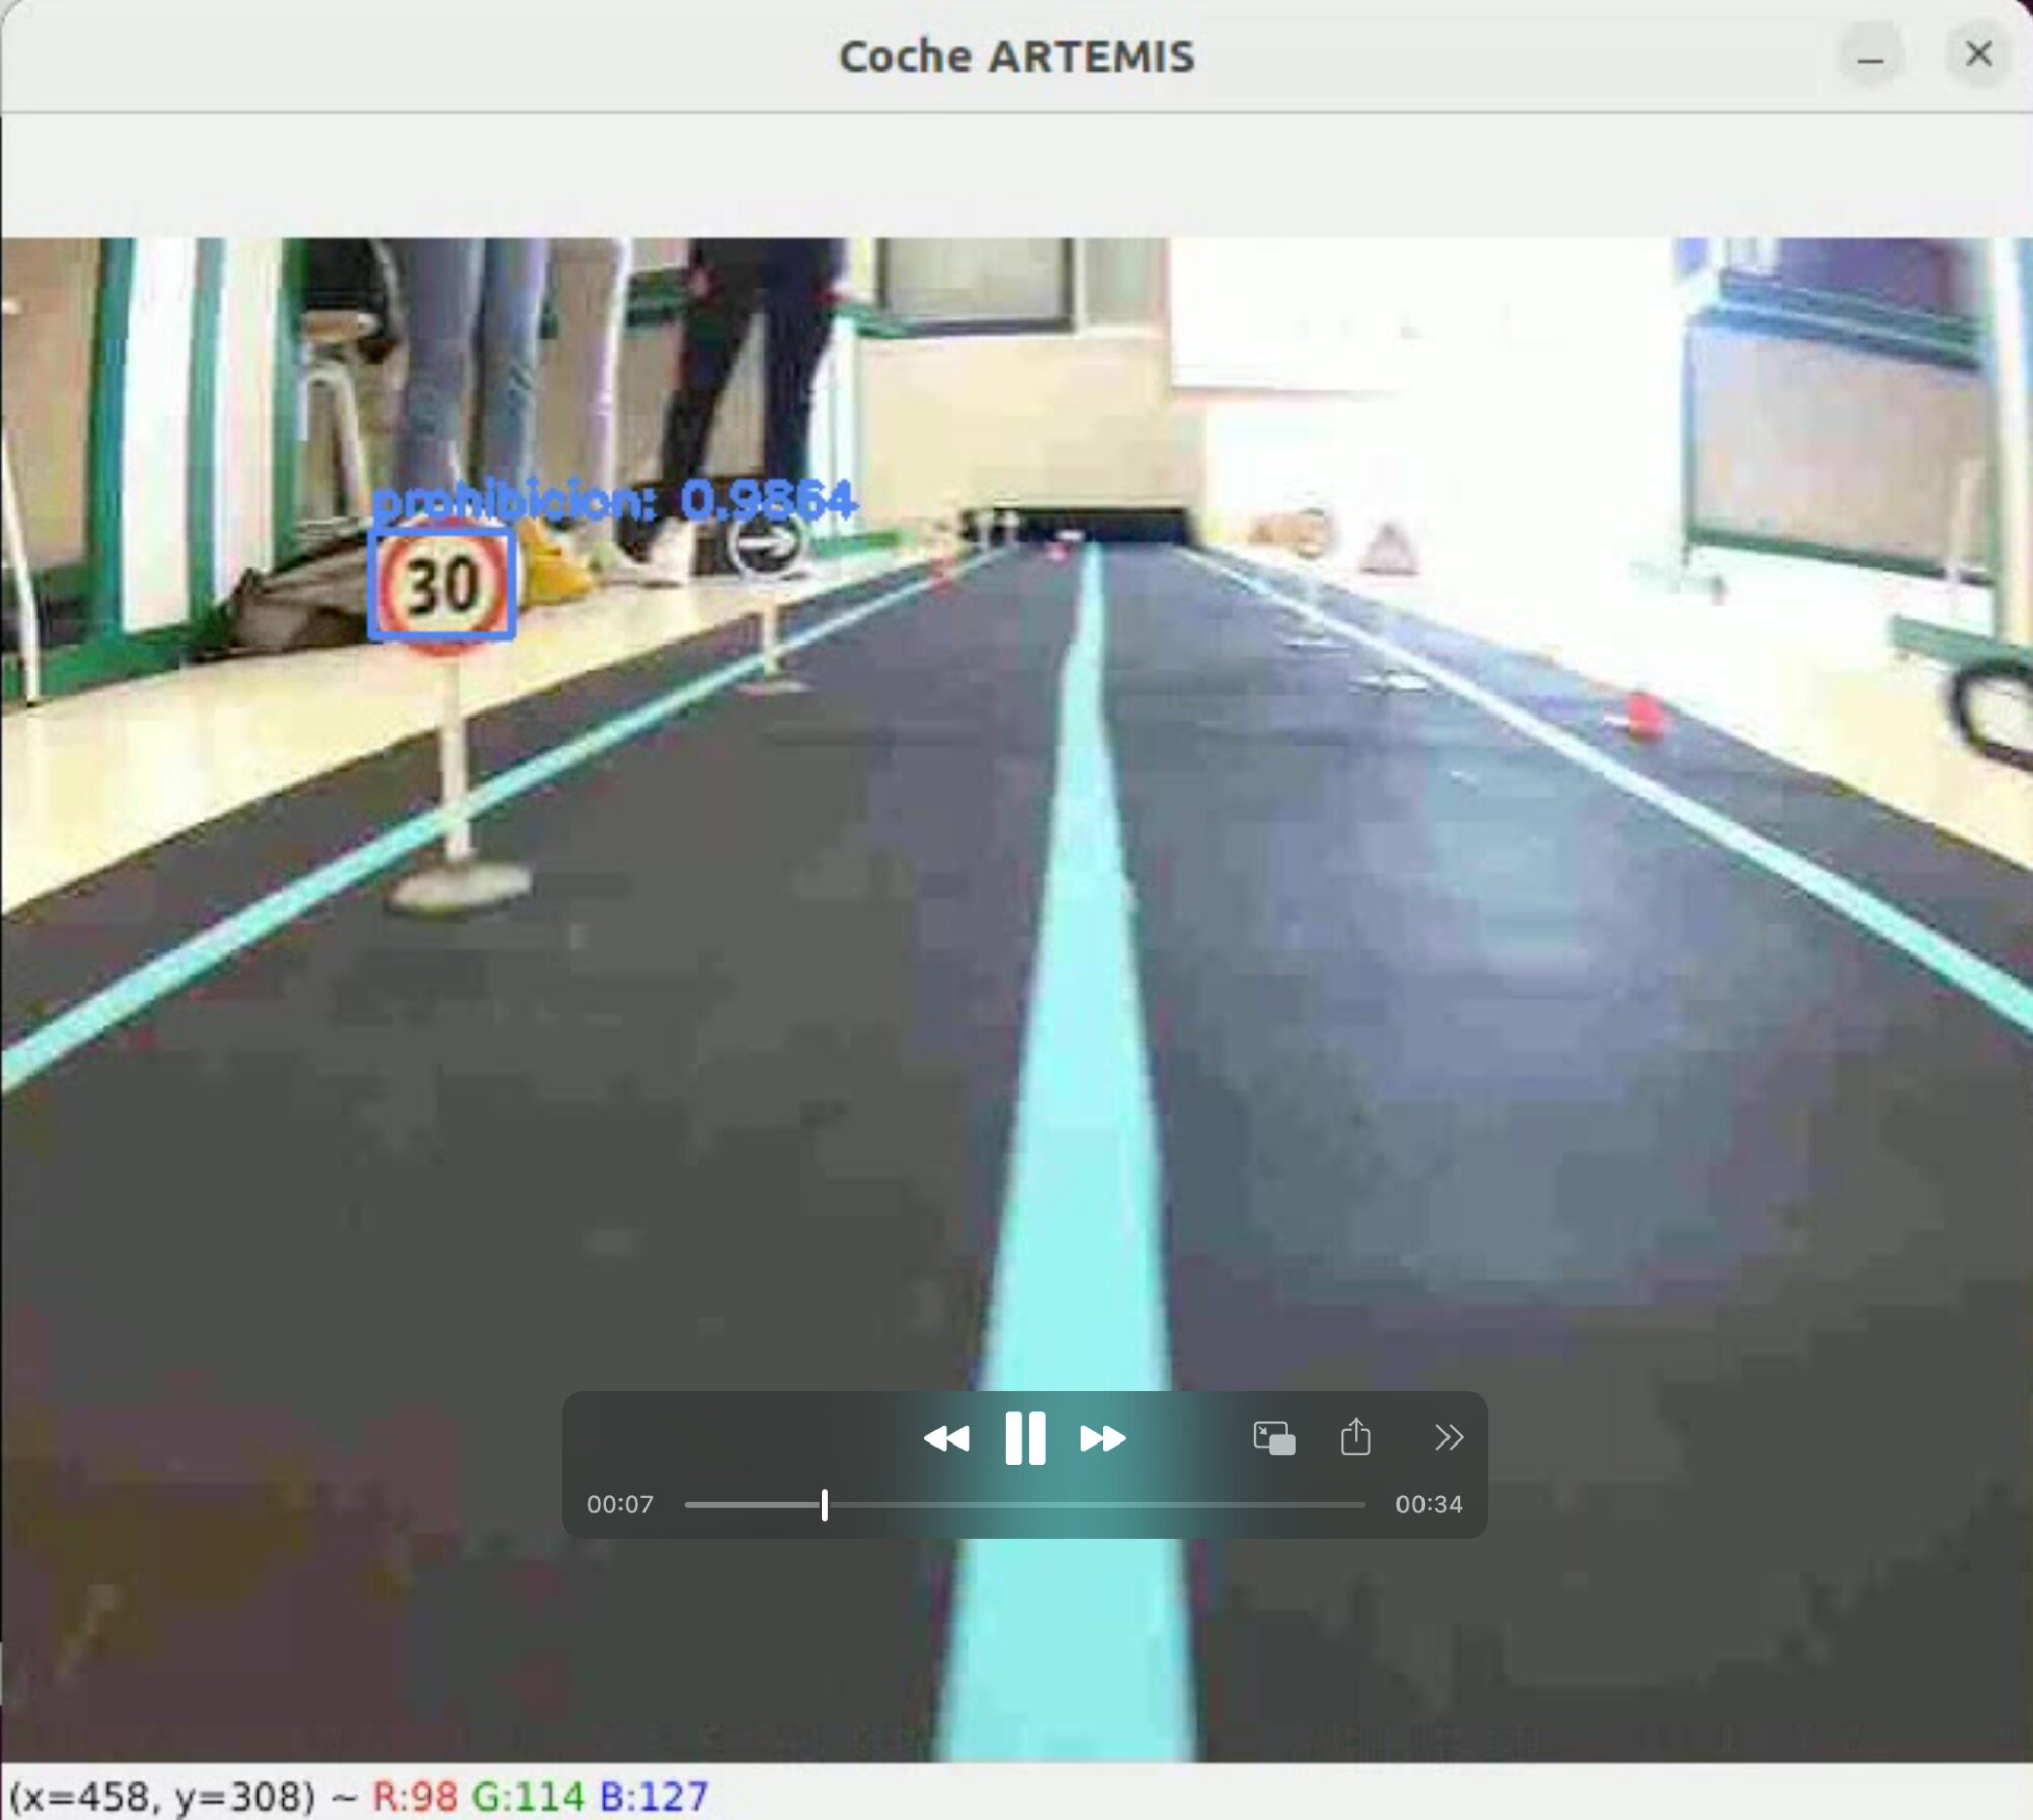
\includegraphics[width=\textwidth]{Imagenes/AnexoI_Manual/AA/deteccion1.pdf}
	\caption{Detección de una señal}
	\label{detecc1}
\end{figure}

En caso de querer realizar el procesamiento de un video, lo haremos con el script \textbf{yolo-3-video.py}. De igual manera debemos modificar la variable \textit{videoName} con el nombre del video, el cual ha de encontrarse dentro de la carpeta \textit{videos} en formato MP4. Lo pondremos en marcha mediante, obteniendo como resultado la figura \ref{detecc2}
\begin{lstlisting}
	python3 video_yolov3.py
\end{lstlisting}
	
\begin{figure}[H]
	\centering
	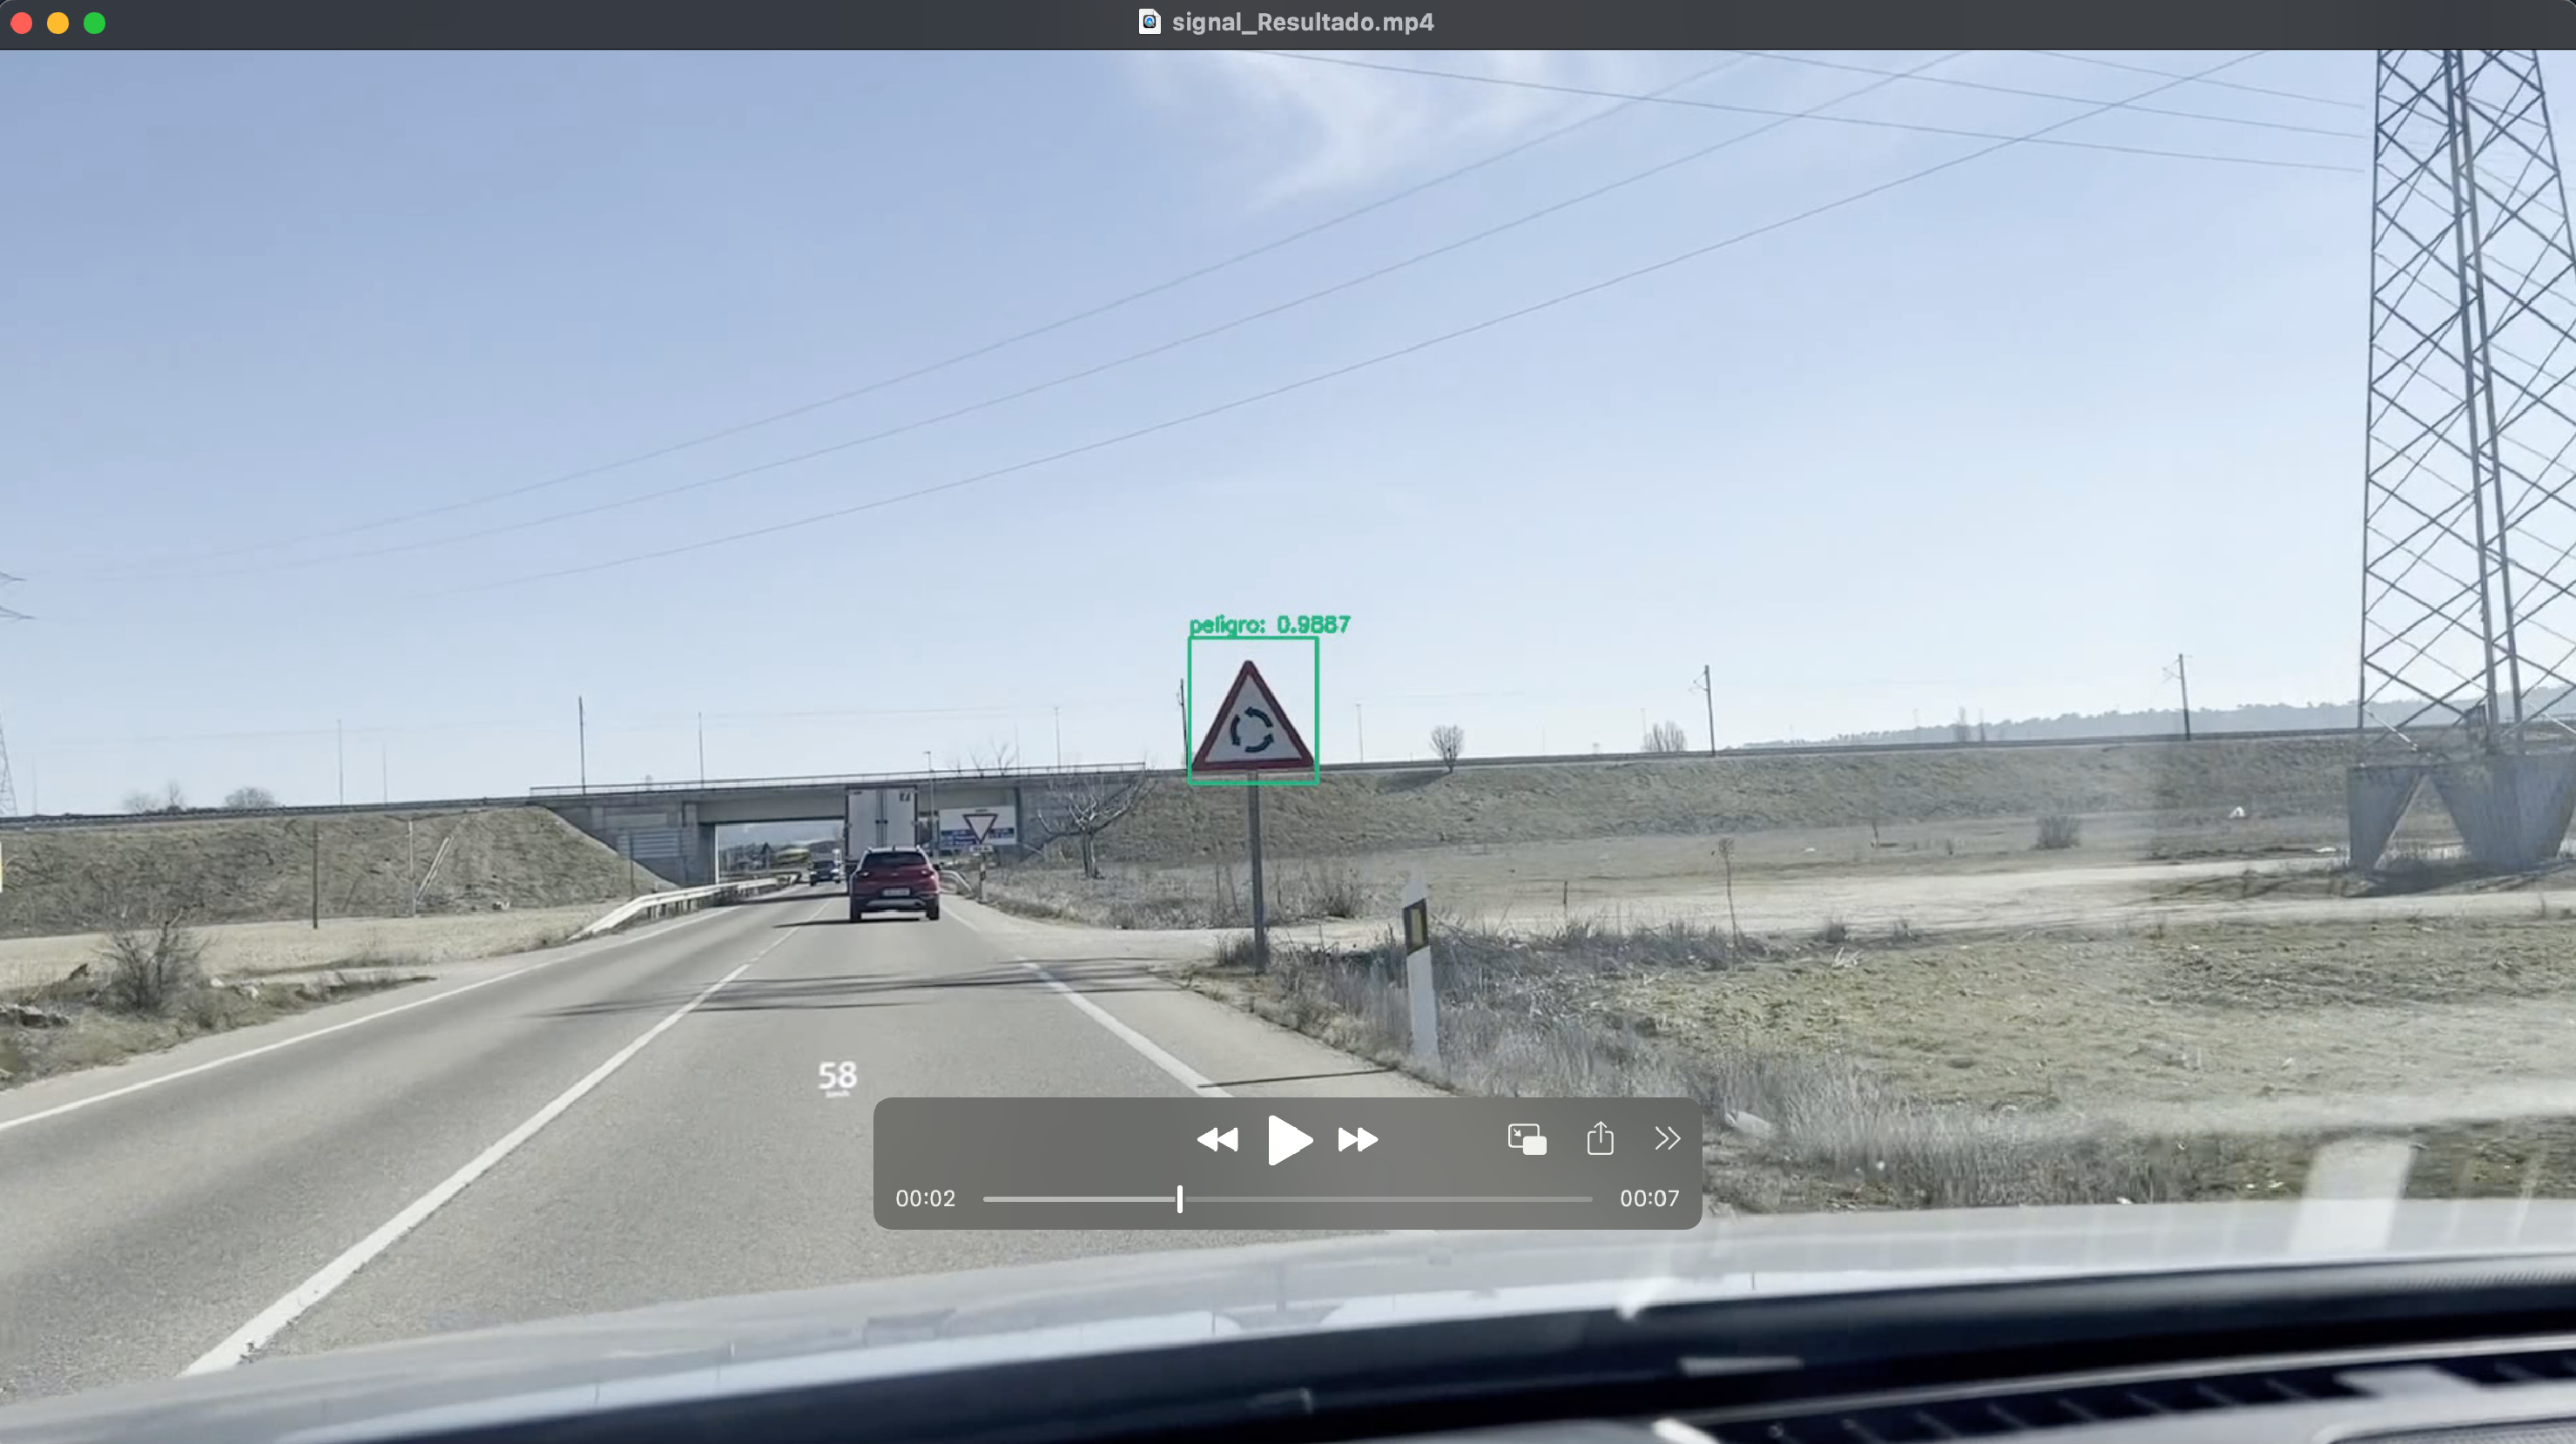
\includegraphics[width=\textwidth]{Imagenes/AnexoI_Manual/AA/deteccion2.pdf}
	\caption{Detección de una señal real capturada por nosotros}
	\label{detecc2}
\end{figure}

Asimismo, podremos procesar video en tiempo real procedente de la cámara o webcam de nuestro propio ordenador, figura \ref{detecc3}. A través del script \textbf{camara_yolov3.py} podremos ponerlo en marcha:

\begin{lstlisting}
python3 camara_yolov3.py
\end{lstlisting}

\begin{figure}[H]
	\centering
	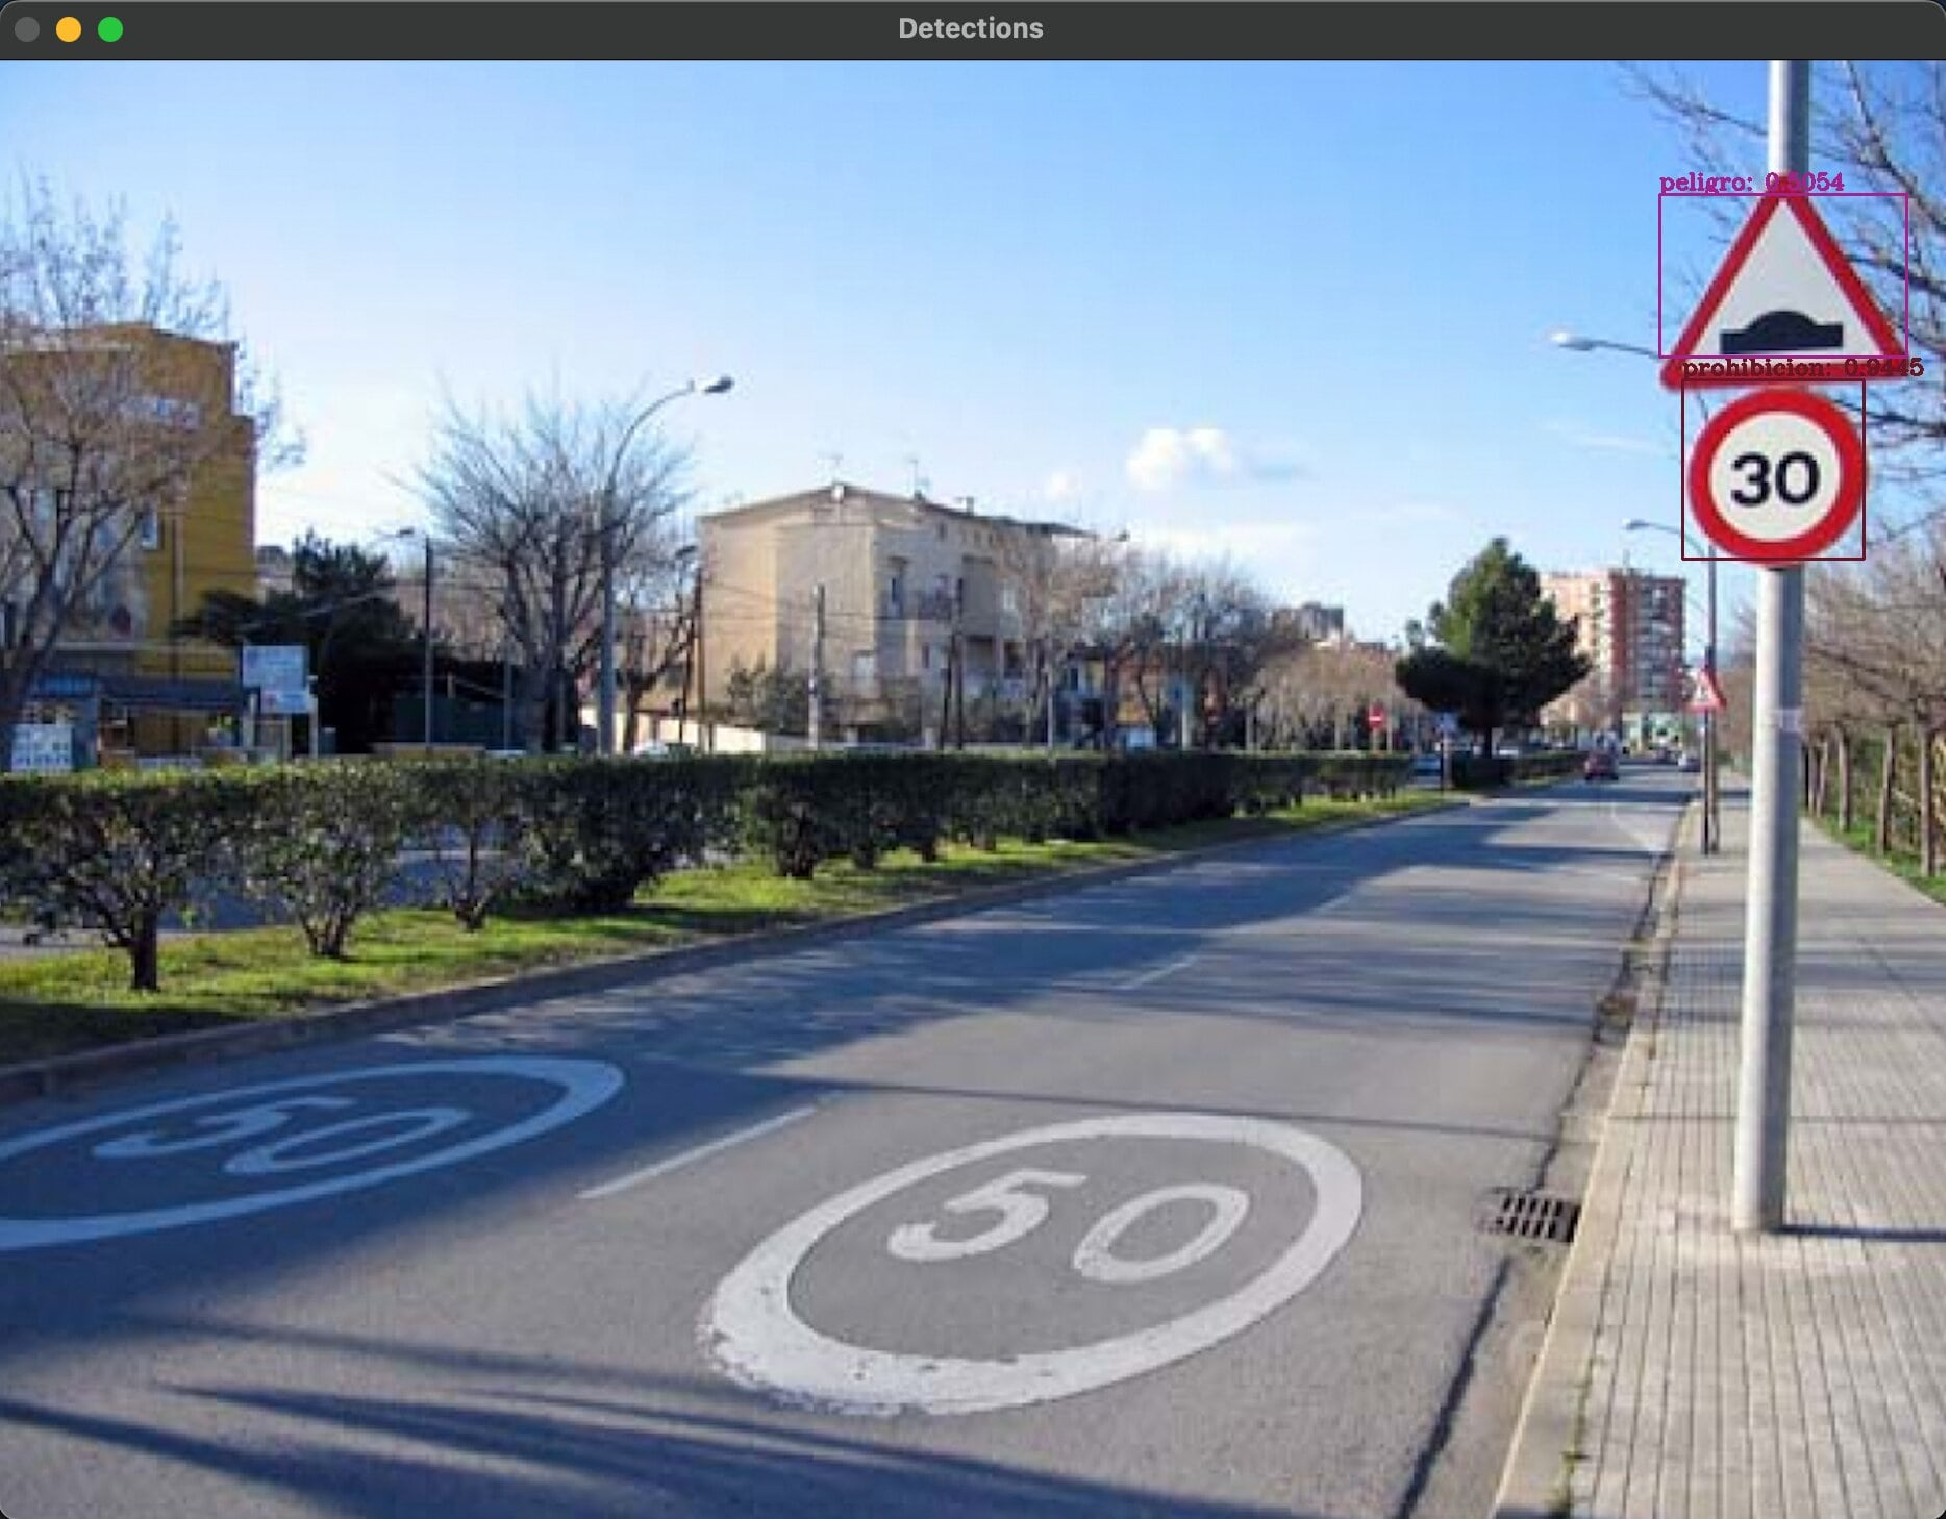
\includegraphics[width=\textwidth]{Imagenes/AnexoI_Manual/AA/deteccion3.pdf}
	\caption{Detección de una señal captada por la cámara}
	\label{detecc3}
\end{figure}

Puede ser de utilidad poder procesar muchas imágenes de manera conjunta, por ejemplo, si quisiéramos medir el rendimiento de la red. Para ello, disponemos de dos scripts que funcionan de manera conjunta, estos son \textbf{automatic_imagen_yolov3.py} y \textbf{automatizacion_imagenes.py}. 

El script que deberemos ejecutar es \textbf{automatizacion_imagenes.py}, el cual leerá cuáles son las imágenes que se encuentran en el directorio especificado en la variable \textit{directorioAutomatic} y ejecutará individualmente \textbf{automatic_imagen_yolov3.py} con el nombre de cada imagen como parámetro de entrada.

Dado que nosotros hemos utilizado dichos scripts para hacernos más sencilla la tarea de medición de rendimiento de la red, tendremos la posibilidad de crear un fichero \textbf{nombre_imagen.txt} por cada imagen, que contendrá las coordenadas del cuadro delimitador del objeto detectado y la precisión obtenida. Mediante la variable que se encuentra al comiendo del fichero \textbf{automatic_imagen_yolov3.py} llamada \textit{medirRendimientoRed} podremos controlar dos modos de operación:

\begin{itemize}
\item Si \textit{medirRendimientoRed} es \textbf{False}: su funcionamiento será análogo al script \textbf{imagen_yolov3.py}, pero podremos visualizar varias imágenes de seguido, simplemente deberemos pulsar cualquier tecla para visualizar la siguiente. 

\item Si \textit{medirRendimientoRed} es \textbf{True}: podremos crear el fichero \textbf{nombre_imagen.txt} con su información correspondiente dentro del directorio \textit{detections} para cada una de las imágenes, pero no iremos viendo en tiempo real el procesado.
\end{itemize}

Mediante la siguiente instrucción podremos ejecutarlo:

\begin{lstlisting}
python3 automatizacion_imagenes.py
\end{lstlisting}

Si además tuviéramos la opción de \textit{medirRendimientoRed} establecida a \textbf{True}, obtendremos un resultado similar al de la figura \ref{detecc4}.

\begin{figure}[H]
	\centering
	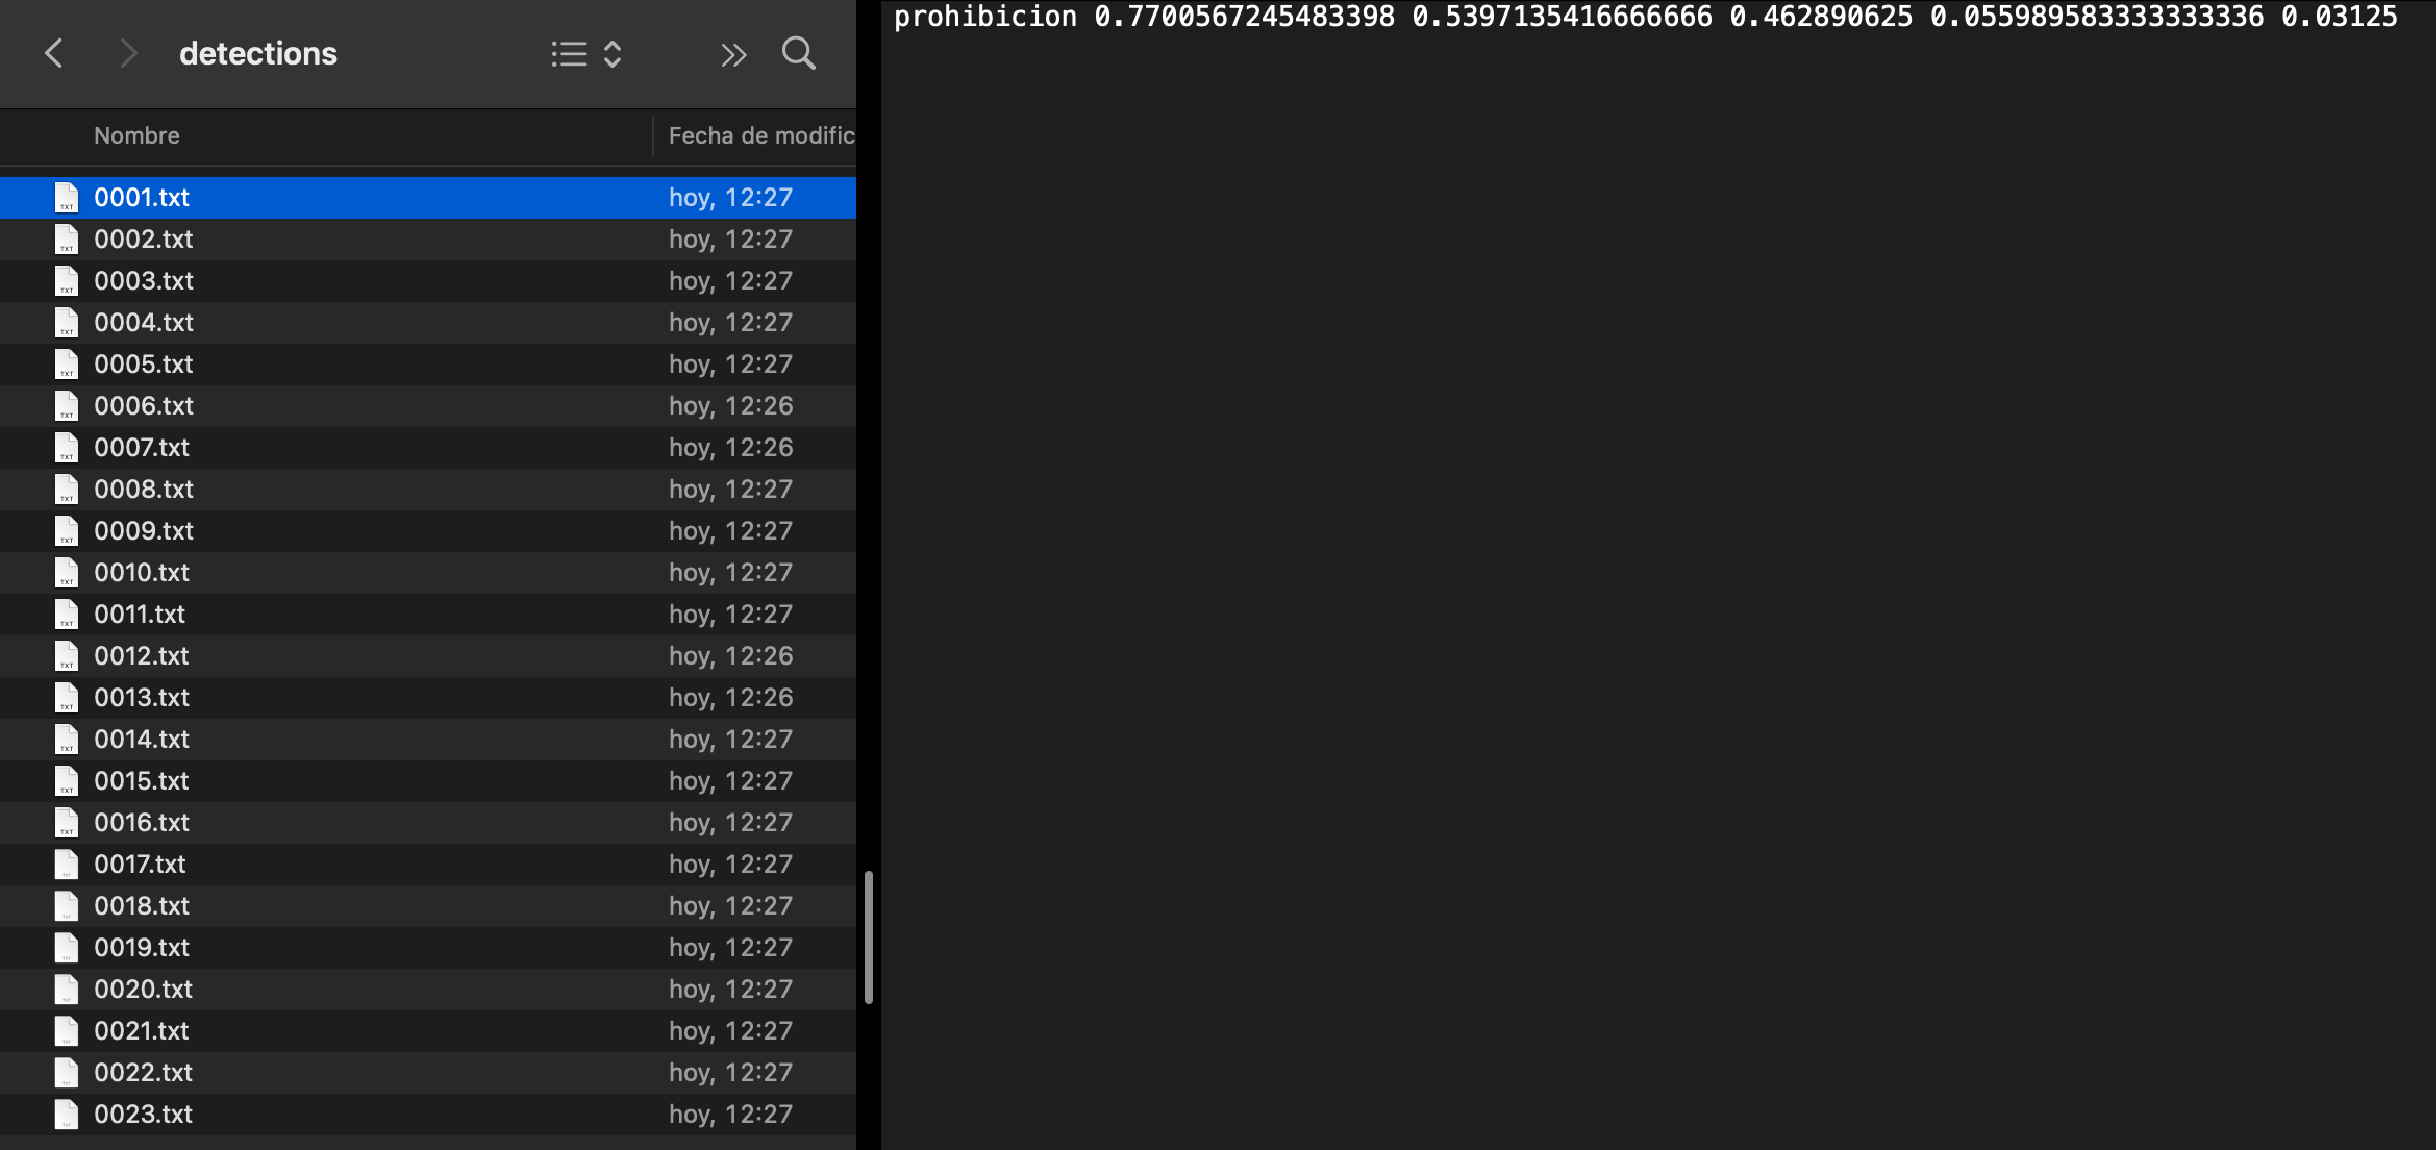
\includegraphics[width=\textwidth]{Imagenes/AnexoI_Manual/AA/deteccion4.pdf}
	\caption{Ejemplo de rendimiento con $medirRendimientoRed \ =\ True$}
	\label{detecc4}
\end{figure}




\subsection{Herramienta de etiquetado}
	Existen números herramientas de etiquetado compatibles con \textbf{YOLO}, pero quizás una de las más sencillas de usar sea \textit{LabelIMG}. Esta herramienta se encuentra disponible tanto para \textit{Windows} como para \textit{MAC OS/Linux}.\\

Para poder acceder a \textit{LabelIMG} se puede hacer a través de su propio repositorio de \textit{GitHub} \url{https://github.com/heartexlabs/labelImg}, el cual presenta las distintas opciones de instalación que se tienen dependiendo de la plataforma. En caso de necesitar instalarla en un ordenador \textit{MAC OS/Linux}, debido a las diferentes incompatibilidades entre librerías con las que nos encontramos en su momento, recomendamos instalar las que se indican en el fichero de \textbf{requirements.txt}. \\

Para hacer uso de dicha herramienta simplemente debemos inicializar su fichero base, el cual lanzará una interfaz con la que interactuaremos para realizar el etiquetado. Para ello, accediendo a la segunda carpeta de nuestro repositorio denominada \textit{2_Etiquetado}, podremos arrancarla:

\begin{lstlisting}
python3 labelImg.py
\end{lstlisting}

Internamente podemos modificar cuáles queremos que sean las clases que por defecto tenemos para etiquetar, en nuestro caso tenemos las diferentes clases de señales: prohibición, peligro, obligación y otros. Si se quisiera modificarlo porque se fuera a utilizar para otra aplicación, se podría modificar mediante el fichero \textbf{predefined_classes.txt} disponible dentro de la carpeta \textit{data}.\\

Se puede trabajar con una imagen individual o con un conjunto de ellas, a través de los botones indicados a continuación podremos abrir las imágenes:

\begin{figure}[H]
	\centering
	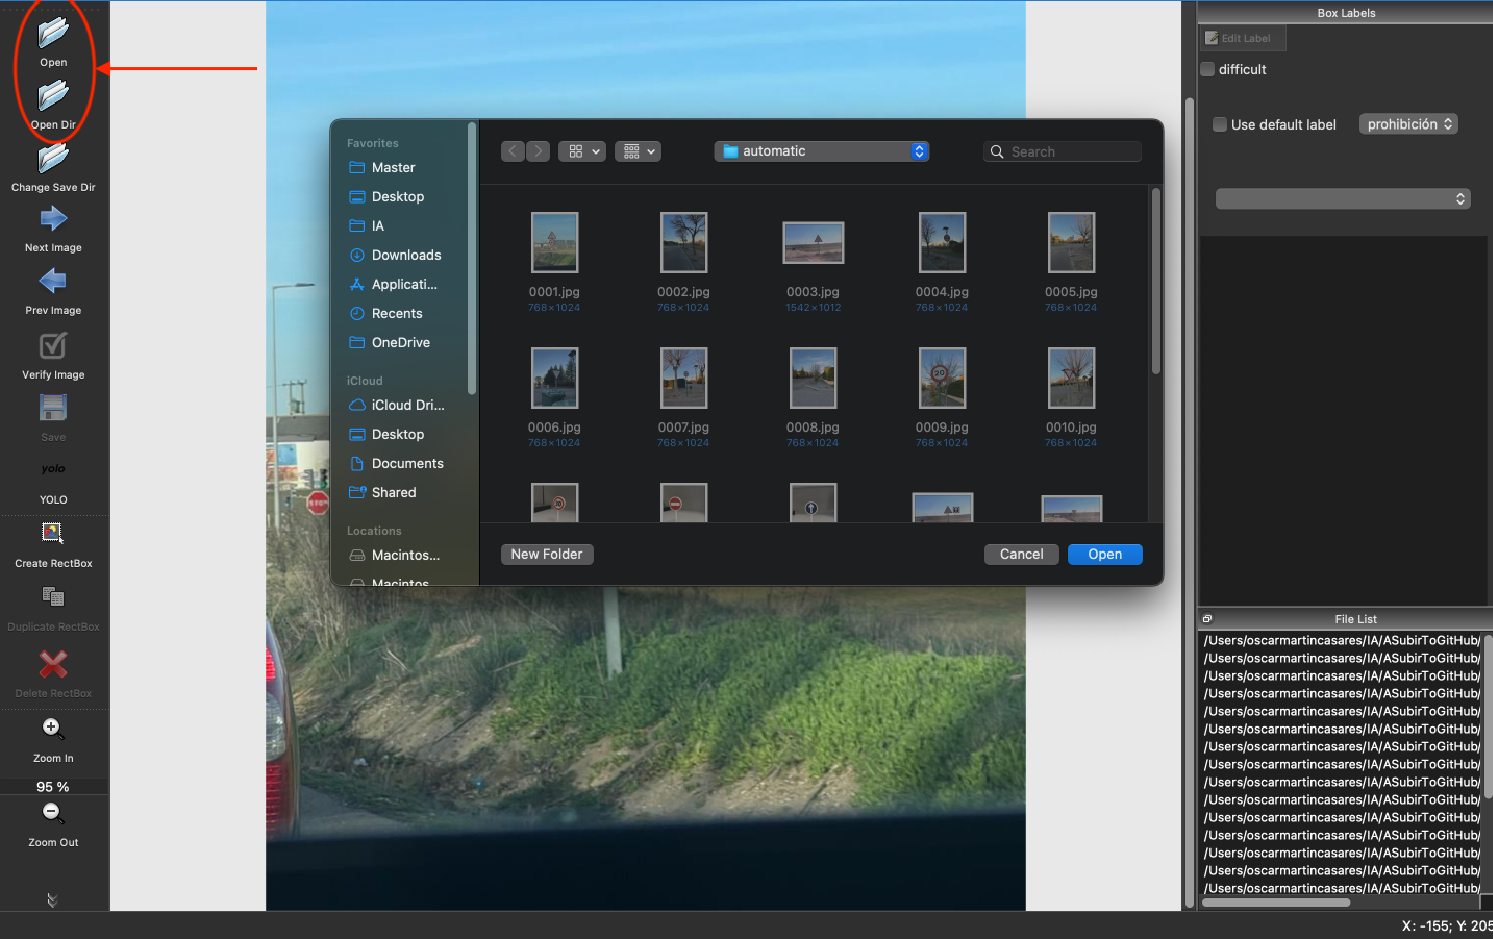
\includegraphics[width=\textwidth]{Imagenes/AnexoI_Manual/AA/etiquetado1.pdf}
	\caption{Etiquetado de una señal}
	\label{etique1}
\end{figure}

Debemos asegurarnos de que el formato en el que se va a producir el etiquetado debe ser únicamente \textbf{YOLO} (ver figura \ref{etique2}. Pulsando sobre el icono mostrado podremos ir intercambiando entre diferentes formatos, ya que esta herramienta es compatible con varios.\\

\begin{figure}[H]
	\centering
	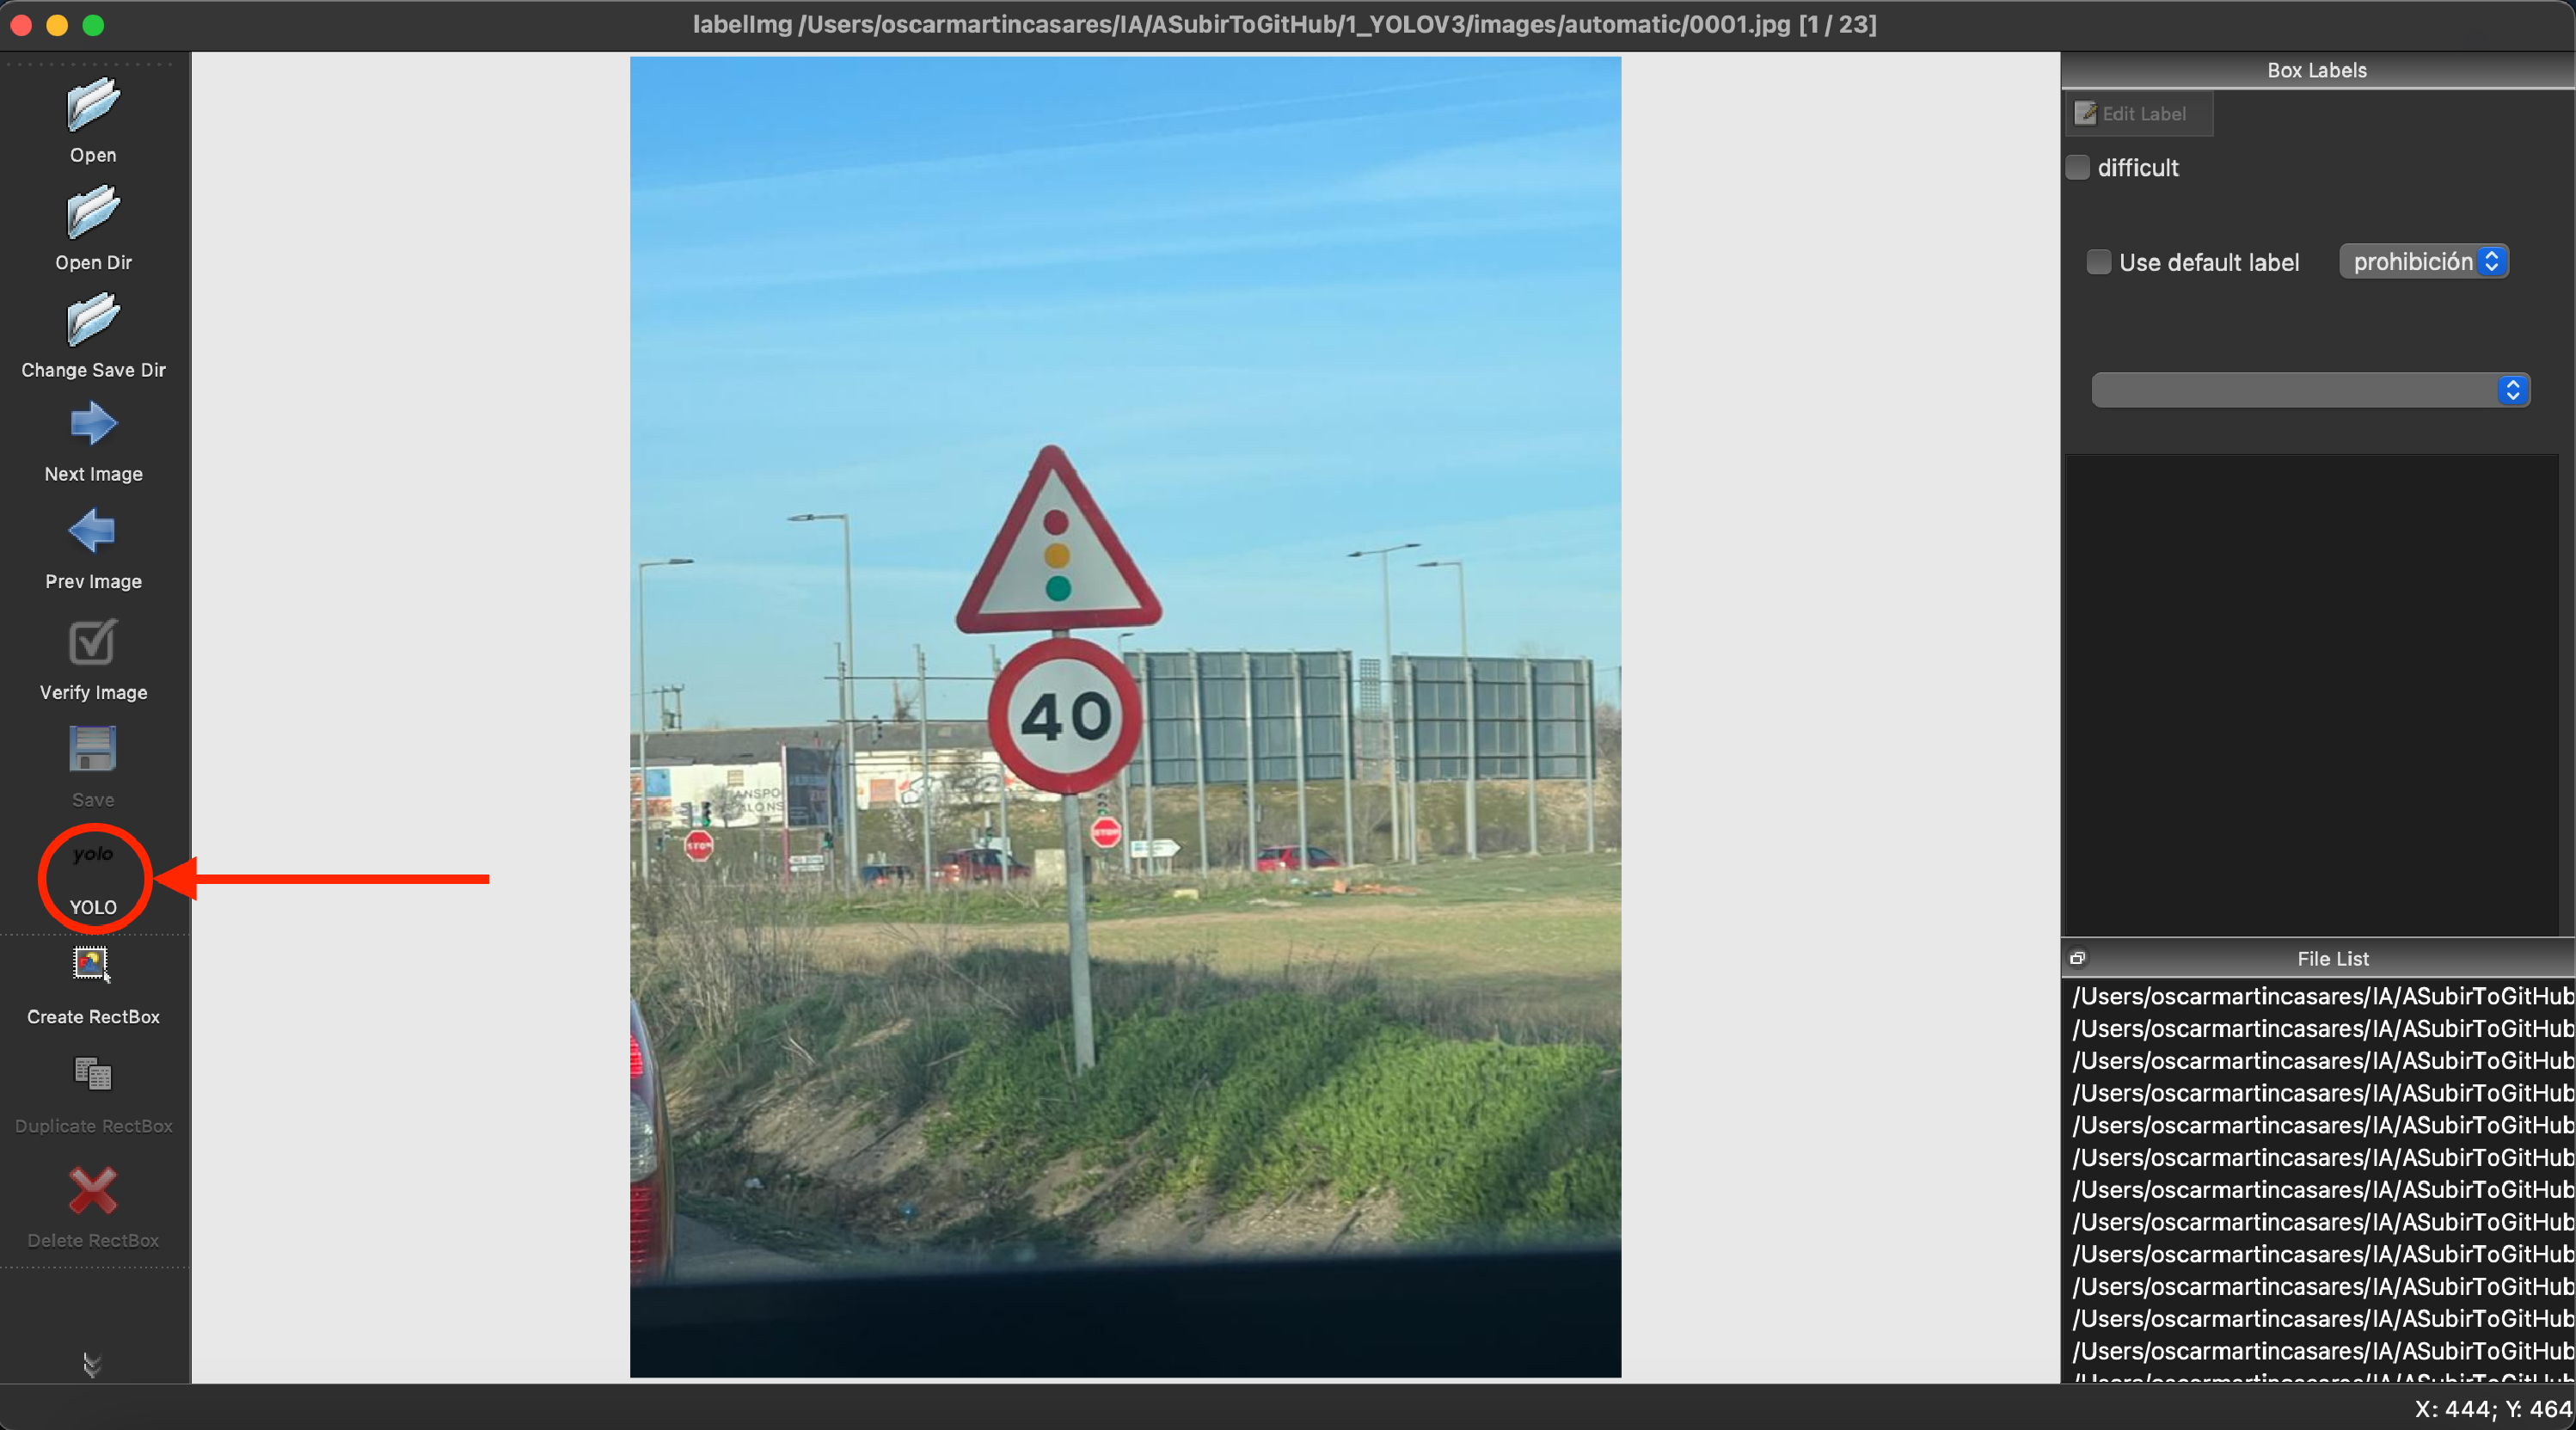
\includegraphics[width=\textwidth]{Imagenes/AnexoI_Manual/AA/etiquetado2.pdf}
	\caption{Selección del modelo}
	\label{etique2}
\end{figure}

Y mediante la opción \textit{Create RectBox} podremos crear los cuadros delimitadores o \textit{bounding boxes} indicando de qué tipo de señal se trata. Ver en la figura \ref{etique3}


\begin{figure}[H]
	\centering
	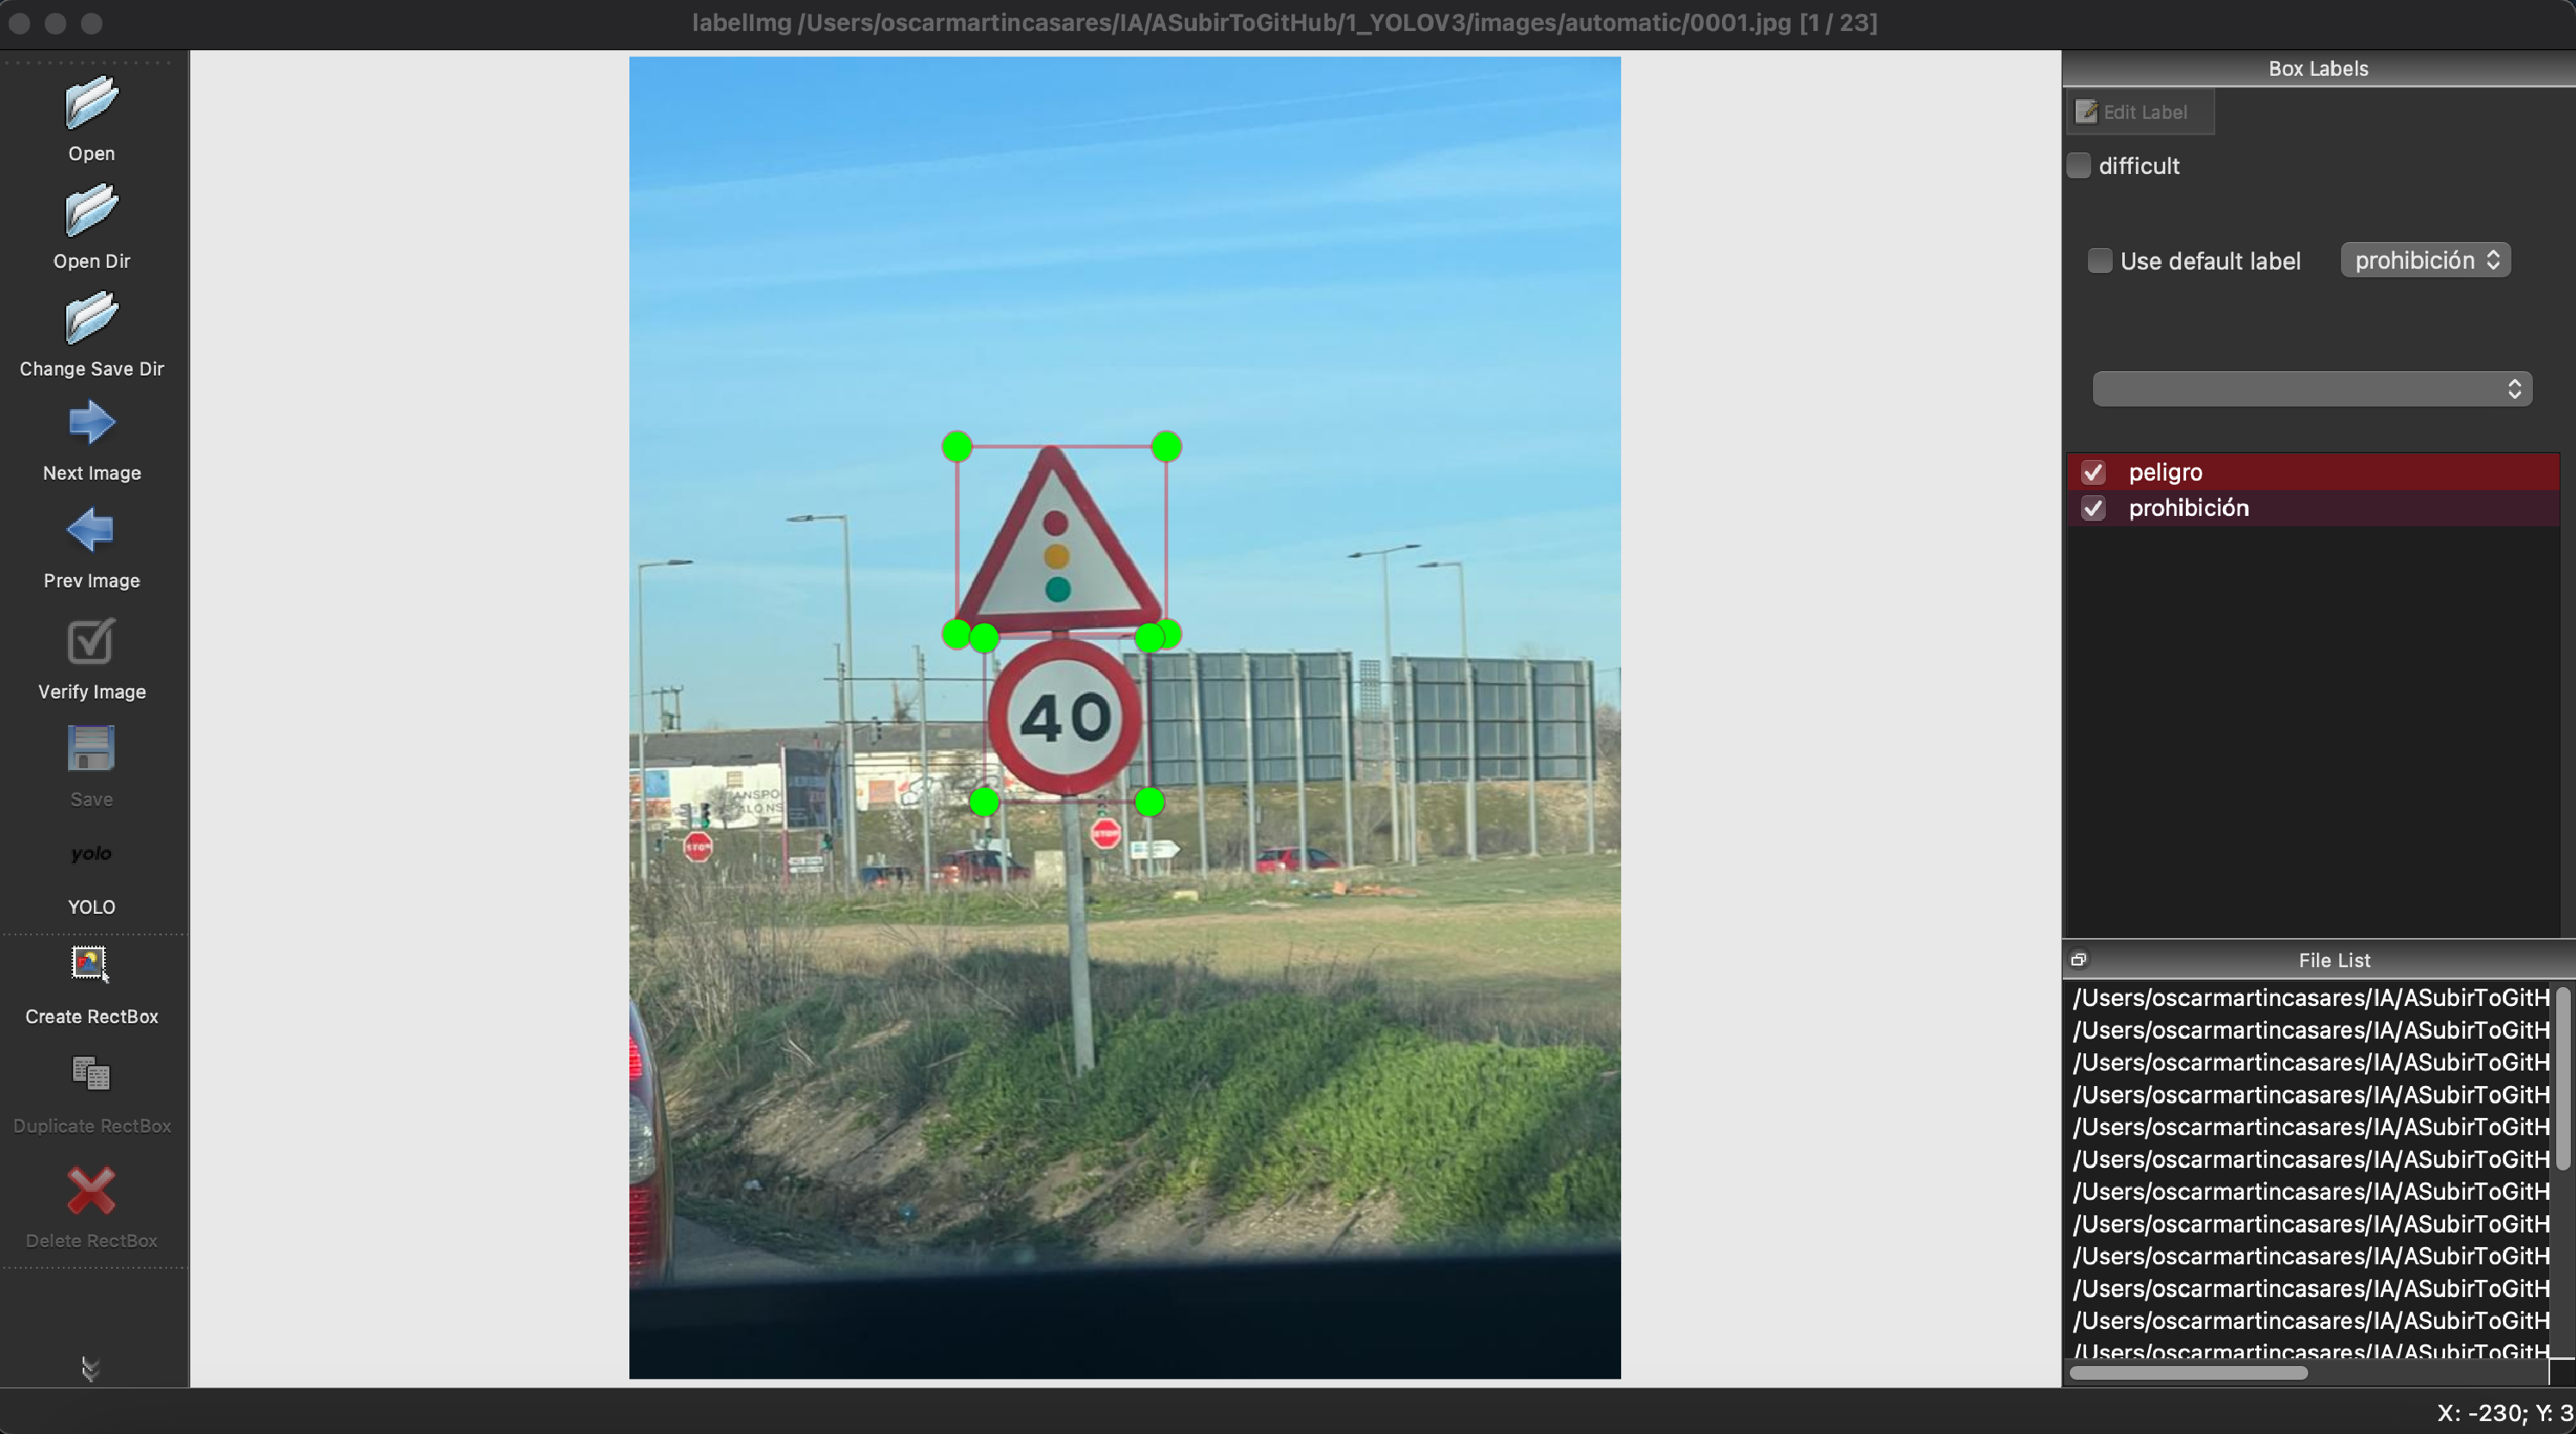
\includegraphics[width=\textwidth]{Imagenes/AnexoI_Manual/AA/etiquetado3.pdf}
	\caption{Cuadros delimitadores}
	\label{etique3}
\end{figure}

Al guardar la imagen se nos creará un fichero en formato \textbf{TXT} que contendrá la información de etiquetado (Figura \ref{etique4}) en el directorio que contenga la imagen en cuestión, con idéntico formato \textbf{YOLO} a como se nos mostraba en detección con la opción \textit{medirRendimientoRed} a \textbf{True}.

\begin{figure}[H]
	\centering
	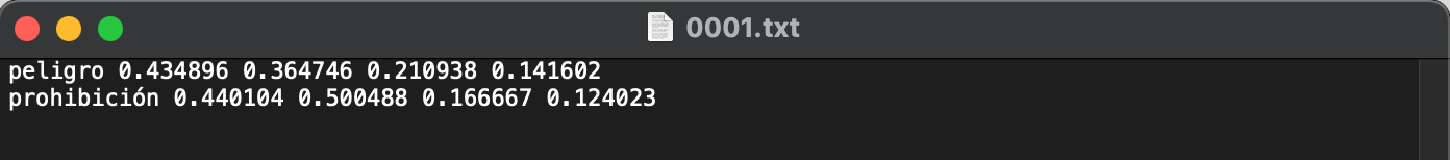
\includegraphics[width=\textwidth]{Imagenes/AnexoI_Manual/AA/etiquetado4.pdf}
	\caption{Fichero con la información de etiquetado}
	\label{etique4}
\end{figure}

Además, creemos de puede ser de utilidad una herramienta que convierta un video a \textit{frames}, para poder etiquetarlos de manera manual para entrenar o cualquier otra aplicación. Esta herramienta se llama \textbf{ffmpeg} \url{https://ffmpeg.org} y se puede instalar de manera muy sencilla mediante el comando: 

\begin{lstlisting}
pip3 install ffmpeg 
\end{lstlisting}

Simplemente desde línea de comandos podremos utilizarla, indicando cuál es el video que queremos dividir, en cuántos \textit{frames} queremos dividirlo y cómo queremos que se llamen cada una de las imágenes. 

\begin{lstlisting}
ffmpeg -i nombre_video.mp4 -vf fps=4 nombre_imagen-%d.jpeg
\end{lstlisting}

	
\subsection{Medición de rendimiento}
	En cuestiones de medición del rendimiento, existe un repositorio de \textit{GitHub} muy popular utilizado por la mayoría de la gente que busca medir el rendimiento de su modelo de inteligencia artificial. Este repositorio es \url{https://github.com/rafaelpadilla/Object-Detection-Metrics.git}, posee un fichero \textbf{README.md} de vital importancia, en el que se explica todas las métricas que podemos obtener, su explicación teórica y cómo obtenerlas. Asimismo, proporciona dos ejemplos guiados para poder realizar pruebas sencillas. En nuestro proyecto se encuentra dentro de la tercera carpeta \textit{3_Rendimiento}.\\

Sin embargo, nosotros hemos realizado nuestro propio script \textbf{precisionVSrecall.py} para poder obtener la curva de Precisión vs Recuperación (\textit{Precision vs Recall}) que se encuentra dentro del directorio rendimiento. Mediante esta curva podremos evaluar el modelo. La precisión se refiere a la proporción de verdaderos positivos (TP) y falsos positivos (FP). La recuperación se refiere a la proporción de verdaderos positivos entre la suma de verdaderos positivos con falsos negativos. En definitiva, sirve para evaluar la calidad de un modelo de clasificación y se puede utilizar para determinar el umbral óptimo para el modelo.\\

La idea principal para obtener dicha curva es comparar la clase y cuadros de delimitadores de numerosas fotos etiquetadas y procesadas por el algoritmo de detección. Es decir, para una imagen comparar la señal real con la detectada. Se deben introducir todos los ficheros TXT con los datos de etiquetado en el interior de \textbf{rendimiento/images/groundtruths/} y los ficheros TXT con los datos de detección en el directorio \textbf{rendimiento/images/detections/}. Ejecutando entonces el script \textbf{precisionVSrecall.py} podremos obtener la curva de rendimiento:
\begin{lstlisting}
python3 precisionVSrecall.py
\end{lstlisting}

A modo de ejemplo, nosotros probamos con 64 imágenes y estos fueron los resultados que obtuvimos:

\begin{figure}[H]
	\centering
	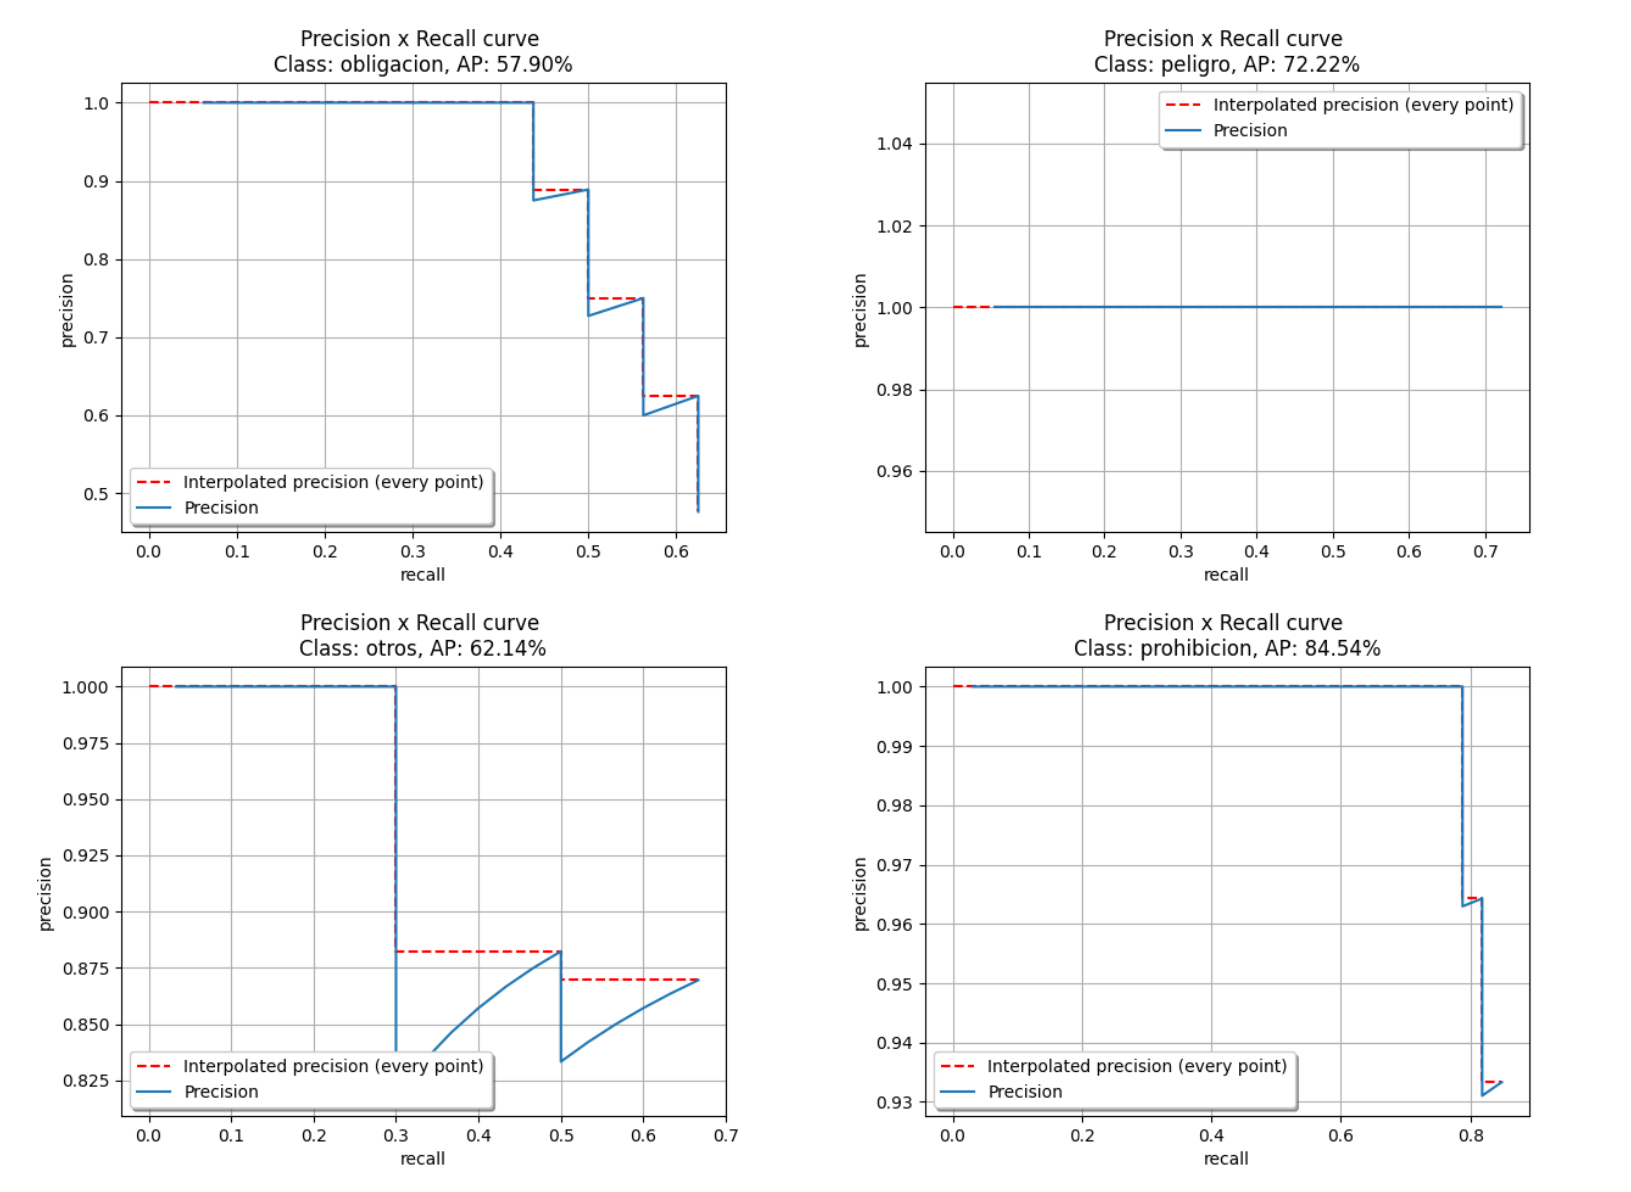
\includegraphics[width=\textwidth]{Imagenes/AnexoI_Manual/AA/rendimiento.pdf}
	\caption{Medida de rendimiento}
	\label{rendimiento2}
\end{figure}




\subsection{Creación automática de datasets}
	Debido a la tarea de creación de datasets es muy tedioso, sobre todo por la tarea de etiquetado, aparte de buscar en Internet datasets realizados por terceros, podemos utilizar una herramienta que nos permite moldear uno a nuestro gusto. Esta herramienta se llama \textbf{OIDv4_ToolKit} \url{https://github.com/EscVM/OIDv4_ToolKit.git} y se encuentra en la cuarta carpeta \textit{4_Crear_Dataset}.\\

En el propio \textit{README.md} de la herramienta se nos explica su funcionamiento, si por ejemplo quisiéramos descargar un dataset que estuviera formado por 8 imágenes de coches y autobuses podríamos hacer:

\begin{lstlisting}
python3 main.py downloader --classes Car Bus --type_csv train --multiclasses 1 --limit 8
\end{lstlisting}

En la figura \ref{dataset} podemos observar como en la carpeta \textit{OID/Dataset/train/Car_Bus/} se nos han descargado las 8 imágenes, incluyendo sus ficheros TXT con la información de etiquetado en el interior de la carpeta \textit{Label}:

\begin{figure}[H]
	\centering
	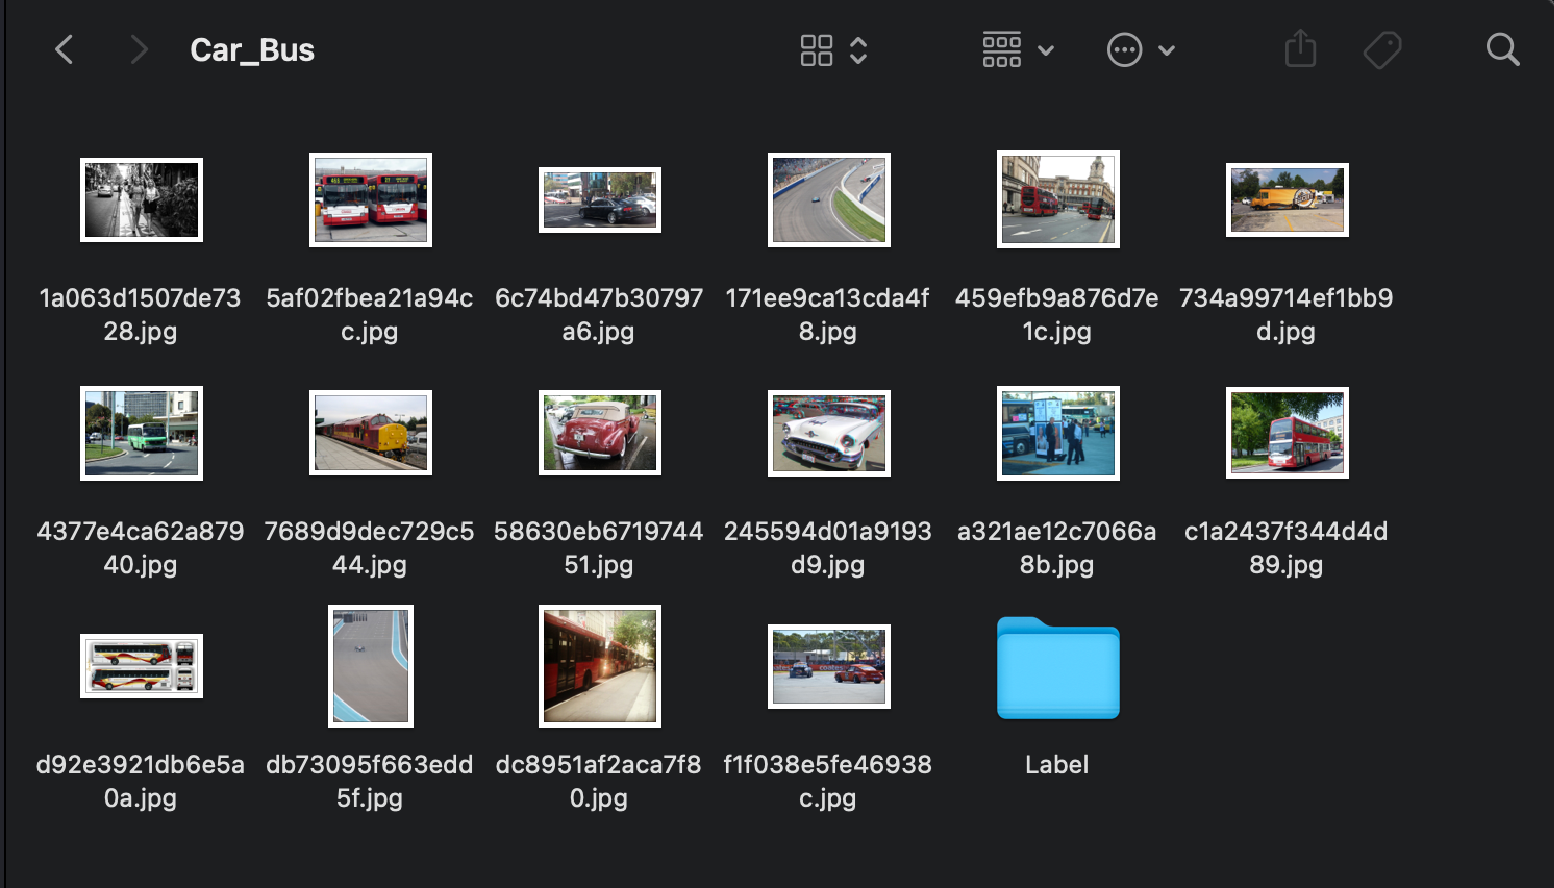
\includegraphics[width=\textwidth]{Imagenes/AnexoI_Manual/AA/dataset.pdf}
	\caption{Dataset descargado con los ficheros TXT}
	\label{dataset}
\end{figure}

Sin embargo, dichos ficheros con la información de etiquetado no se encuentran en formato \textbf{YOLO}, por lo que habrá que realizar la transformación. Dicha tarea se puede llevar a cabo mediante el script que se encuentra dentro de la herramienta \textbf{OIDv4_ToolKit} llamado \textbf{convert_to_YOLO.py}. \\

En dicho \textit{script} debemos cambiar introducir dos rutas, la que contiene las imágenes descargadas y en la que se encuentra el fichero CSV con todas las clases disponibles para descargar en la herramienta. Para obtener dichas rutas se pueden con un \textit{script} tan sencillo como este:

\begin{lstlisting}
import os
current_dir = os.path.dirname(os.path.abspath(__file__))
print(current_dir)
\end{lstlisting}

Tras ejecutar el \textit{script} podremos observar como en el directorio en el que se encuentran las imágenes se han creado cada uno de los ficheros TXT con el mismo nombre con la información de etiquetado \textbf{YOLO}. Podríamos comprobar además si se ha realizado con éxito la transformación abriendo dicho directorio con la herramienta de etiquetado \textbf{LabelImg}.

